\documentclass[handout]{beamer}
%==============================================================
% Common Beamer Preamble for Course Lectures: Training and Scaling Language Models
%==============================================================

\usepackage[utf8]{inputenc}
\usepackage[T1]{fontenc}
\usepackage{hyperref}
\usepackage{amsmath,amssymb,xcolor,multicol,booktabs,colortbl}
\usepackage{graphicx,listings}
\renewcommand{\figurename}{Figure.}
\renewcommand{\tablename}{Table.}

% ---- TikZ Libraries ----
\usepackage{tikz}
\usetikzlibrary{positioning,arrows.meta,shapes.geometric,calc,fit,backgrounds,decorations.pathreplacing}

% ---- Presentation defaults ----
\setbeamertemplate{navigation symbols}{}
\setbeamersize{text margin left=0.55cm,text margin right=0.55cm}
\setbeamerfont{title}{size=\LARGE,series=\bfseries}
\setbeamerfont{subtitle}{size=\large}

% ---- FontAwesome fallback ----
\IfFileExists{fontawesome5.sty}{%
  \usepackage{fontawesome5}%
}{%
  \providecommand{\faMicrochip}{}%
  \providecommand{\faComments}{}%
  \providecommand{\faTools}{}%
  \providecommand{\faCheckCircle}{}%
  \providecommand{\faExclamationTriangle}{}%
  \providecommand{\faImage}{}%
  \providecommand{\faRobot}{}%
  \providecommand{\faTerminal}{}%
  \providecommand{\faBook}{}%
  \providecommand{\faRedo}{}%
  \providecommand{\faLayerGroup}{}%
  \providecommand{\faCogs}{}%
  \providecommand{\faDatabase}{}%
  \providecommand{\faHdd}{}%
  \providecommand{\faNetworkWired}{}%
}

% ---- Theme Style and Semantic Colors ----
%==============================================================
% Centralized Semantic Color Definitions for LLMs Presentation
%==============================================================

% ---- Base Template / Theme Colors (Aligned with Palette B) ----
\definecolor{themenavy}{RGB}{22,70,102}       % Palette B primary cerulean: #164666
\definecolor{themeblue}{RGB}{22,70,102}       % Primary alias
\definecolor{primarylight}{RGB}{34,92,132}    % Primary light: #225c84
\definecolor{themeteal}{RGB}{0,159,176}       % Accent cyan-teal: #009fb0
\colorlet{main_color}{themenavy}
\colorlet{accent}{themeteal}

\definecolor{accentdark}{RGB}{0,108,120}      % Deep cyan-teal for contrast text
\definecolor{accentlight}{RGB}{56,178,214}    % Slate accent cyan: #38b2d6
\definecolor{leafred}{RGB}{197,93,61}         % Terracotta red for branches/leaves

% ---- Website Panel & Border Neutrals ----
\definecolor{panelbg}{RGB}{237,245,249}       % Course-panel: #edf5f9
\definecolor{panelborder}{RGB}{204,226,238}   % Course-border: #cce2ee

% ---- Code listing style (syntax highlights) ----
\definecolor{deepblue}{RGB}{22,70,102}
\definecolor{deepred}{rgb}{0.6,0,0}
\definecolor{deepgreen}{RGB}{0,135,150}
\definecolor{halfgray}{gray}{0.55}

% ---- Semantic Theme Navy / Cerulean Shades ----
\colorlet{themebluebg}{panelbg}               % Panel #edf5f9
\colorlet{themebluecard}{main_color!8}        % Mild card background fills
\colorlet{themeblueborder}{panelborder}       % Border #cce2ee
\colorlet{themebluemid}{themeteal!60}         % Accent mid-contrast
\colorlet{themebluedraw}{main_color!80}       % Strong outline draws/strokes

% ---- Semantic Secondary Accent Teal Shades ----
\colorlet{accentdarkbg}{themeteal!10}        % Light secondary background fills
\colorlet{accentdarkdraw}{themeteal}         % Secondary outlines/strokes/text/axes

% ---- Functional Colors: Success Green ----
\definecolor{successgreen}{RGB}{55,145,55}
\colorlet{successbg}{successgreen!8}
\colorlet{successdraw}{successgreen!75}

% ---- Functional Colors: Alert Red ----
\definecolor{alertred}{RGB}{197,55,55}
\colorlet{alertbg}{alertred!8}
\colorlet{alertdraw}{alertred!75}

% ---- Functional Colors: Warning Orange ----
\definecolor{warningorange}{RGB}{220,110,30}
\colorlet{warningbg}{warningorange!10}
\colorlet{warningdraw}{warningorange!80}

% ---- Terracotta Red Shades ----
\colorlet{leafredbg}{leafred!12}
\colorlet{leafreddraw}{leafred!80}

% ---- Accent Violet (SWE-bench / observe phases) ----
\definecolor{accentviolet}{RGB}{120,70,180}
\colorlet{accentvioletbg}{accentviolet!10}
\colorlet{accentvioletdraw}{accentviolet!80}

% ---- Post-Training Axis Blue ----
\definecolor{posttrainingblue}{RGB}{40,90,165}
\colorlet{posttrainingbg}{posttrainingblue!8}
\colorlet{posttrainingdraw}{posttrainingblue!75}

% ---- Harness Component Action Green ----
\definecolor{actiongreen}{RGB}{55,145,55}
\colorlet{actiongreenbg}{actiongreen!10}
\colorlet{actiongreendraw}{actiongreen!65}

% ---- Harness Component Persist Olive ----
\definecolor{persistolive}{RGB}{120,135,40}
\colorlet{persistolivebg}{persistolive!12}
\colorlet{persistolivedraw}{persistolive!70}

% ---- Harness Component Observe Violet ----
\colorlet{observevioletbg}{accentvioletbg}
\colorlet{observevioletdraw}{accentvioletdraw}

% ---- Neutrals (Grays/Blacks) ----
\colorlet{neutralbg}{black!4}             % Very light background fills
\colorlet{neutrallight}{black!30}         % Border frames/ticks/dividers
\colorlet{neutraldark}{black!75}          % Main body text/code listing text

% ---- Beamer Block Color Overrides (Premium Terracotta Theme) ----
\setbeamercolor{block title alert}{bg=leafreddraw,fg=white}
\setbeamercolor{block body alert}{bg=leafredbg}
\setbeamercolor{alerted text}{fg=leafreddraw}

\usepackage{../common/style}
\graphicspath{{../common/figs/}{figs/}}

% ---- Code Listing Config ----
\lstset{
  basicstyle=\ttfamily\footnotesize,
  keywordstyle=\bfseries\color{deepblue},
  emphstyle=\ttfamily\color{deepred},
  stringstyle=\color{deepgreen},
  commentstyle=\color{halfgray}\itshape,
  numbers=left, numberstyle=\tiny\color{halfgray},
  backgroundcolor=\color{codebg},
  frame=l, framerule=1.5pt, rulecolor=\color{themeteal},
  xleftmargin=10pt, framexleftmargin=4pt, numbersep=6pt,
  showstringspaces=false, breaklines=true,
  aboveskip=4pt, belowskip=4pt
}

% ---- Image Placeholder Utility ----
\newcommand{\slideimage}[2][3.8cm]{%
  \begin{center}
    \begin{tikzpicture}
      \node[draw=main_color, dashed, very thick, rounded corners,
        fill=themebluebg, minimum width=0.88\linewidth, minimum height=#1,
      text width=0.80\linewidth, align=center, font=\itshape, text=accentdark]
      {\textbf{[ FIGURE / DIAGRAM ]}\\[6pt] #2};
    \end{tikzpicture}
  \end{center}
}

% ---- Concept Highlight Card Utility ----
\newcommand{\conceptcard}[3]{%
  \begin{coursebox}{#1}{#2}#3
  \end{coursebox}%
}

% ---- Reusable teaching-slide components ----
\newcommand{\learninggoals}[4]{%
  \begin{frame}{What should be clear by the end?}
    \begin{enumerate}
        \setlength{\itemsep}{7pt}
      \item #1
      \item #2
      \item #3
      \item #4
    \end{enumerate}
  \end{frame}
}

\newcommand{\checkpoint}[2]{%
  \begin{frame}{Checkpoint: #1}
    \begin{block}{Think, then compare}
      #2
    \end{block}
  \end{frame}
}

\newcommand{\takeaways}[4]{%
  \begin{frame}{Key takeaways}
    \begin{enumerate}
        \setlength{\itemsep}{8pt}
      \item #1
      \item #2
      \item #3
      \item #4
    \end{enumerate}
  \end{frame}
}

\newcommand{\smallsource}[1]{%
  \vfill\hfill{\tiny\color{neutraldark}Source: #1}
}

% ---- Logo on content frames ----
\newif\ifplacelogo
\placelogotrue
\logo{\ifplacelogo
  \raisebox{-0.3ex}{
\includegraphics[height=0.4cm]{IMT_Atlantique_logo.png}}%
\fi}

\makeatletter
\define@key{beamerframe}{nologo}[true]{%
  \placelogofalse
}
\makeatother

% Fix Beamer bold font warning: substitute undefined T1/cmss/b/n with T1/cmss/bx/n
\DeclareFontShape{T1}{cmss}{b}{n}{<->ssub * cmss/bx/n}{}

% Default Author, Institute & Date metadata
\author[BRAIN team]{BRAIN team}
\institute[IMT Atlantique]{IMT Atlantique}
\date{January 2027}

% Override \date so individual decks calling \date{\today} do not overwrite the common date
\renewcommand{\date}[2][]{}

% ---- Front Page / Title Slide Macro ----
% Displays Title + IMT Atlantique logo and Brain logo
\newcommand{\makelecturetitle}[1][Training and Scaling Language Models: From First Principles to Efficient Serving]{%
  \placelogofalse
  {
    \setbeamertemplate{footline}{}
    \settitletagline{#1}
    \settitlelogos{%
      \raisebox{-0.5\height}{
\includegraphics[height=1.15cm]{IMT_Atlantique_logo.png}}%
      \hspace{1.2em}%
    \raisebox{-0.5\height}{\includegraphics[height=1.15cm]{brain.pdf}}}
    \def\insertauthor{BRAIN team}
    \def\insertdate{January 2027}
    \begin{frame}[plain]
      \titlepage
    \end{frame}
  }
  \placelogotrue
}

% Section TOC Frame
\AtBeginSection[]{\coursesectiondivider}

% Shared two-GPU visual grammar for the parallelism lectures.
\tikzset{
  parallel device/.style={draw=themebluedraw!65,fill=themebluebg!25!white,
    sharp corners,line width=.65pt,minimum width=5.0cm,minimum height=2.0cm,
    align=center,font=\footnotesize},
  parallel exchange/.style={draw=accentdarkdraw,fill=accentdarkbg,
    sharp corners,line width=.7pt,minimum width=7.5cm,minimum height=.68cm,
    align=center,font=\small\bfseries},
  parallel connection/.style={line width=.8pt,draw=accentdarkdraw},
}
% One outlined bar is a conceptual tensor, split into two logical partitions.
% Explicit sharp corners prevent device-node styling leaking into nested TikZ.
\newcommand{\ParallelFull}[1]{\tikz[baseline=-.55ex,x=.50cm,y=.25cm,sharp corners]{\path[sharp corners,fill=#1] (0,0) rectangle (2,1);\draw[sharp corners,draw=#1,line width=.5pt] (0,0) rectangle (2,1);\draw[sharp corners,white,line width=.5pt] (1,0)--(1,1);}}
\newcommand{\ParallelLeft}[1]{\tikz[baseline=-.55ex,x=.50cm,y=.25cm,sharp corners]{\path[sharp corners,fill=#1] (0,0) rectangle (1,1);\path[sharp corners,fill=white] (1,0) rectangle (2,1);\draw[sharp corners,draw=#1,line width=.5pt] (0,0) rectangle (2,1);\draw[sharp corners,draw=#1,line width=.5pt] (1,0)--(1,1);}}
\newcommand{\ParallelRight}[1]{\tikz[baseline=-.55ex,x=.50cm,y=.25cm,sharp corners]{\path[sharp corners,fill=white] (0,0) rectangle (1,1);\path[sharp corners,fill=#1] (1,0) rectangle (2,1);\draw[sharp corners,draw=#1,line width=.5pt] (0,0) rectangle (2,1);\draw[sharp corners,draw=#1,line width=.5pt] (1,0)--(1,1);}}
% Aligned columns keep the same position for state and activation glyphs on both devices.
\newcommand{\ParallelCardTwo}[5]{%
  \begin{tabular}{@{}l@{\hspace{6pt}}l@{}}
    \multicolumn{2}{@{}l}{\textbf{#1}}\\[6pt]
    #2 & #3\\[5pt]
    #4 & #5
  \end{tabular}%
}
\newcommand{\ParallelCardThree}[7]{%
  \begin{tabular}{@{}l@{\hspace{6pt}}l@{}}
    \multicolumn{2}{@{}l}{\textbf{#1}}\\[5pt]
    #2 & #3\\[4pt]
    #4 & #5\\[4pt]
    #6 & #7
  \end{tabular}%
}
\newcommand{\ParallelLegend}{%
  {\scriptsize \textcolor{themenavy}{\rule{7pt}{7pt}\ model state}\quad
  \textcolor{leafreddraw}{\rule{7pt}{7pt}\ data / activations}\quad
  \textcolor{accentdark}{\rule{7pt}{7pt}\ communication}\quad outline = held elsewhere}%
}

\title[TASLLM -- Module 5]{Module 5: Distributed Data Parallelism\\[4pt]
\normalsize\itshape Replicas, Collectives, and Global Invariants}
\date{\today}

\begin{document}
\makelecturetitle
\begin{frame}{Lecture map}
  \tableofcontents
  \vfill
  \begin{block}{Guiding question}
    When does training on $W$ GPUs reproduce one larger-batch update, and where can that equivalence fail?
  \end{block}
\end{frame}
\learninggoals
{Explain ranks, process groups, collective communication and its costs.}
{Derive DDP gradient averaging and connect it to accumulation.}
{Keep accumulation, sampling, logging, and checkpointing rank-aware.}
{Measure both numerical equivalence and scaling efficiency.}

\section{Distributed foundations}

\begin{frame}{Why go beyond one GPU?}
  \begin{columns}[t]
    \begin{column}{.47\linewidth}
      \begin{block}{Throughput}
        Divide work across devices to process a fixed workload sooner, or increase the workload per update.
      \end{block}
    \end{column}
    \begin{column}{.47\linewidth}
      \begin{block}{Capacity}
        Distribute model state or computation when the model and its training state do not fit on one device.
      \end{block}
    \end{column}
  \end{columns}
  \vfill
  \begin{alertblock}{The new cost}
    GPUs must exchange information. Network time, synchronization and changing the global batch can limit or change the result.
  \end{alertblock}
  \small DDP first: replicate the model and split the data. FSDP next: shard model state.
\end{frame}

\begin{frame}{A distributed job: nodes, ranks and process groups}
  \centering
  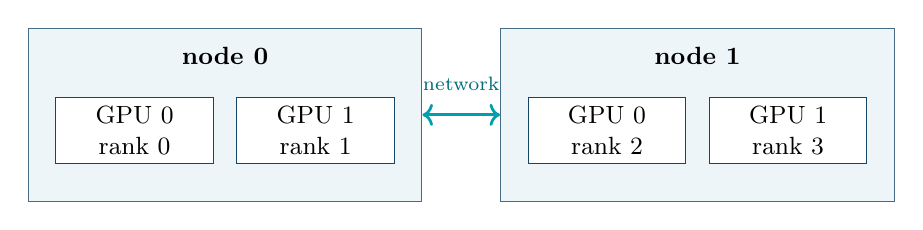
\begin{tikzpicture}[
    every node/.style={font=\small,align=center},
    host/.style={draw=themebluedraw,fill=themebluebg,minimum width=5cm,minimum height=2.2cm},
    device/.style={draw=themenavy,fill=white,minimum width=2cm,minimum height=.75cm},
    link/.style={line width=1pt,draw=accentdarkdraw}]
    \node[host] (n0) at (-3,0) {};
    \node[host] (n1) at (3,0) {};
    \node[font=\small\bfseries] at (-3,.75) {node 0};
    \node[font=\small\bfseries] at (3,.75) {node 1};
    \node[device] at (-4.15,-.2) {GPU 0\\rank 0};
    \node[device] at (-1.85,-.2) {GPU 1\\rank 1};
    \node[device] at (1.85,-.2) {GPU 0\\rank 2};
    \node[device] at (4.15,-.2) {GPU 1\\rank 3};
    \draw[link,<->] (n0.east)--(n1.west);
    \node[font=\scriptsize,text=accentdark] at (0,.4) {network};
  \end{tikzpicture}
  \vfill
  \small One process per GPU in standard DDP. \textbf{Global rank} identifies a process; \textbf{local rank} identifies its GPU on the node. A \textbf{process group} defines who communicates. Here the world size is 4.
\end{frame}

\begin{frame}{All-reduce: sum corresponding entries on every rank}
  \definecolor{rankteal}{HTML}{BDECEE}
  \definecolor{rankamber}{HTML}{FDE68A}
  \definecolor{rankviolet}{HTML}{E9D5FF}
  \definecolor{rankrose}{HTML}{FECDD3}
  \centering
  \begin{tikzpicture}[x=1cm,y=1cm,scale=.70,transform shape,every node/.style={font=\scriptsize,align=center}]
    % The same color throughout a column identifies the contributing rank.
    \node[anchor=east,font=\small\bfseries,text=themeink] at (-5.2,2.55) {Local input};
    \node[anchor=east,font=\small\bfseries,text=themeink] at (-5.2,-.42) {Reduced output};
    \foreach \x/\r/\c in {-3.9/0/rankteal,-1.3/1/rankamber,1.3/2/rankviolet,3.9/3/rankrose} {
      \node[font=\small\bfseries,text=themeink] at (\x,3.3) {rank \r};
      \fill[\c] (\x-.9,2.2) rectangle (\x+.9,2.95);
      \draw[themeink!45,thin] (\x-.9,2.2) rectangle (\x+.9,2.95);
      \draw[themeink!30,thin] (\x,2.2)--(\x,2.95);
      \node[font=\small,text=themeink] at (\x-.45,2.58) {$a_{\r}$};
      \node[font=\small,text=themeink] at (\x+.45,2.58) {$b_{\r}$};
      % Each output element contains contributions from all four input ranks.
      \foreach \k/\colour in {0/rankteal,1/rankamber,2/rankviolet,3/rankrose} {
        \pgfmathsetmacro{\leftx}{\x-.9+\k*.225}
        \pgfmathsetmacro{\rightx}{\x-.9+(\k+1)*.225}
        \fill[\colour] (\leftx,-.8) rectangle (\rightx,-.05);
        \pgfmathsetmacro{\leftx}{\x+\k*.225}
        \pgfmathsetmacro{\rightx}{\x+(\k+1)*.225}
        \fill[\colour] (\leftx,-.8) rectangle (\rightx,-.05);
      }
      \draw[themeink!45,thin] (\x-.9,-.8) rectangle (\x+.9,-.05);
      \draw[themeink!30,thin] (\x,-.8)--(\x,-.05);
      \node[font=\small\bfseries,text=themeink] at (\x-.45,-.43) {$\Sigma a$};
      \node[font=\small\bfseries,text=themeink] at (\x+.45,-.43) {$\Sigma b$};
    }
    \node[draw=accentdarkdraw,fill=accentdarkbg,minimum width=5.2cm,minimum height=.55cm,font=\small\bfseries,text=accentdark] (reduce) at (0,.78) {all-reduce: elementwise sum};
    \draw[-{Stealth[length=5pt,width=4pt]},thick,draw=accentdarkdraw] (0,2.05)--(reduce.north);
    \draw[-{Stealth[length=5pt,width=4pt]},thick,draw=accentdarkdraw] (reduce.south)--(0,.02);
    \node[font=\scriptsize,text=neutraldark] at (0,-1.18) {$\Sigma a=\sum_{r=0}^{3}a_r$ \quad and \quad $\Sigma b=\sum_{r=0}^{3}b_r$};
  \end{tikzpicture}
  \par\vspace{4pt}
  \small\textbf{DDP:} divide the sum by the world size to obtain the mean gradient.\par
  \smallsource{NVIDIA NCCL User Guide, Collective Operations}
\end{frame}

\begin{frame}{Communication has a cost}
  \begin{columns}[t]
    \begin{column}{.47\linewidth}
      \begin{block}{Startup and bandwidth}
        Many small messages pay repeated startup costs. Large messages also depend on effective link bandwidth and topology.
      \end{block}
    \end{column}
    \begin{column}{.47\linewidth}
      \begin{block}{Overlap}
        Communication can run while independent GPU work continues. Only the unhidden portion adds directly to the critical path.
      \end{block}
    \end{column}
  \end{columns}
  \vfill
  \begin{alertblock}{Ask of every distributed design}
    What is sent, between which ranks, how often, and what computation can overlap it?
  \end{alertblock}
\end{frame}

\section{The data-parallel contract}

\begin{frame}{From gradient accumulation to data parallelism}
  \begin{columns}[t]
    \begin{column}{.46\linewidth}
      \centering\textbf{One GPU: sequential}\\[-2pt]
      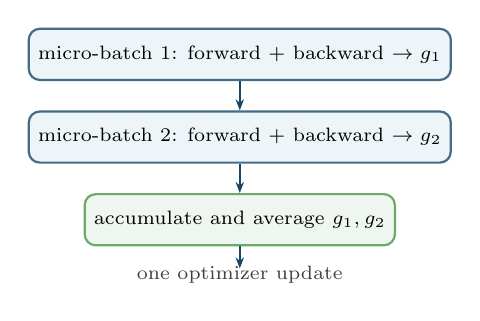
\begin{tikzpicture}[
          every node/.style={font=\scriptsize,align=center},
          box/.style={draw=themebluedraw,fill=themebluebg,rounded corners,minimum width=3.55cm,minimum height=.65cm,thick},
        arr/.style={-{Stealth[length=4pt,width=3pt]},thick,draw=themenavy}]
        \node[box] (a) at (0,2.45) {micro-batch 1: forward + backward $\to g_1$};
        \node[box] (b) at (0,1.40) {micro-batch 2: forward + backward $\to g_2$};
        \node[box,draw=successdraw,fill=successbg] (c) at (0,.35) {accumulate and average $g_1,g_2$};
        \draw[arr] (a)--(b); \draw[arr] (b)--(c);
        \node[font=\scriptsize,text=neutraldark] at (0,-.35) {one optimizer update};
        \draw[arr] (c.south)--++(0,-.28);
      \end{tikzpicture}
    \end{column}
    \begin{column}{.50\linewidth}
      \centering\textbf{Two GPUs: in parallel}\\[-2pt]
      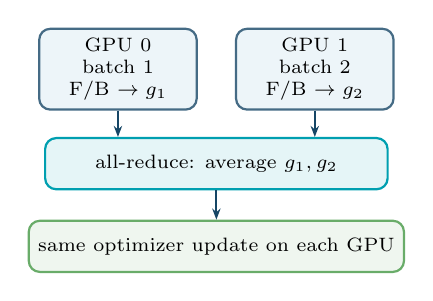
\begin{tikzpicture}[
          every node/.style={font=\scriptsize,align=center},
          box/.style={draw=themebluedraw,fill=themebluebg,rounded corners,minimum width=2.0cm,minimum height=.95cm,thick},
        arr/.style={-{Stealth[length=4pt,width=3pt]},thick,draw=themenavy}]
        \node[box] (a) at (-1.25,2.15) {GPU 0\\batch 1\\F/B $\to g_1$};
        \node[box] (b) at (1.25,2.15) {GPU 1\\batch 2\\F/B $\to g_2$};
        \node[draw=accentdarkdraw,fill=accentdarkbg,rounded corners,minimum width=4.35cm,minimum height=.65cm,thick] (reduce) at (0,.95) {all-reduce: average $g_1,g_2$};
        \node[draw=successdraw,fill=successbg,rounded corners,minimum width=4.35cm,minimum height=.65cm,thick] (step) at (0,-.10) {same optimizer update on each GPU};
        \draw[arr] (a.south)--(a.south |- reduce.north);
        \draw[arr] (b.south)--(b.south |- reduce.north);
        \draw[arr] (reduce)--(step);
      \end{tikzpicture}
    \end{column}
  \end{columns}
  \vspace{2pt}
  \begin{block}{Same global mean gradient}
    \centering $\displaystyle\bar g=\frac{g_1+g_2}{2}$ \qquad (equal-sized micro-batches, same starting weights)
  \end{block}
  {\scriptsize F/B = forward + backward. DDP communicates gradients and keeps model/optimizer replicas. Randomness or batch-dependent operations can affect equivalence.}
\end{frame}

\begin{frame}{Parallelism map: DDP splits the batch}
  \centering
  \ParallelLegend\par\vspace{6pt}
  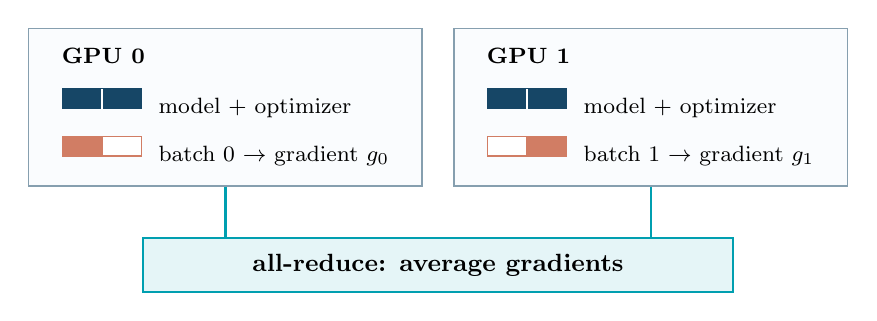
\begin{tikzpicture}
    \node[parallel device] (g0) at (-2.7,0) {\ParallelCardTwo{GPU 0}
      {\ParallelFull{themenavy}}{model + optimizer}
    {\ParallelLeft{leafreddraw}}{batch 0 $\to$ gradient $g_0$}};
    \node[parallel device] (g1) at (2.7,0) {\ParallelCardTwo{GPU 1}
      {\ParallelFull{themenavy}}{model + optimizer}
    {\ParallelRight{leafreddraw}}{batch 1 $\to$ gradient $g_1$}};
    \node[parallel exchange] (comm) at (0,-2.0) {all-reduce: average gradients};
    \draw[parallel connection] (g0.south) -- (g0.south |- comm.north);
    \draw[parallel connection] (g1.south) -- (g1.south |- comm.north);
  \end{tikzpicture}
  \par\vspace{10pt}
  \begin{minipage}{.92\linewidth}\small\raggedright
    \textbf{What changes?}     Different data on each device; the model and optimizer are replicated. After synchronization, every replica applies the same update.
  \end{minipage}\par\vspace{4pt}
  {\scriptsize Equal-size batches; identical initial model and optimizer state.}
\end{frame}

\begin{frame}{Each rank owns a full model and different examples}
  \begin{columns}[c]
    \begin{column}{0.53\linewidth}
      \begin{itemize}
          \setlength{\itemsep}{7pt}
        \item one process controls one GPU
        \item parameters begin identical on all ranks
        \item local batches are disjoint parts of a global batch
        \item gradients synchronize before every optimizer update
      \end{itemize}
    \end{column}
    \begin{column}{0.43\linewidth}
      \begin{block}{Global batch}
        \[
          B_{\text{global}}=W\,B_{\text{local}}\,K
        \]
        $K$ is the number of accumulated micro-steps.
      \end{block}
    \end{column}
  \end{columns}
\end{frame}

\begin{frame}{Gradient averaging recovers the global mean}
  Rank $r$ computes a mean gradient over $n_r$ valid tokens:
  \[
    g_r=\frac{1}{n_r}\sum_{i\in\mathcal{B}_r}\nabla_\theta \ell_i
  \]
  If every $n_r=n$, DDP's average is:
  \[
    \bar g=\frac{1}{W}\sum_{r=0}^{W-1}g_r
    =\frac{1}{Wn}\sum_{r,i}\nabla_\theta\ell_i
  \]
  \begin{alertblock}{Unequal valid-token counts}
    Averaging rank means is not the global token mean. Aggregate summed loss and counts, or weight gradients correctly.
  \end{alertblock}
\end{frame}

\section{Overlap and rank-aware state}

\begin{frame}{Accumulation should synchronize once per update}
  \begin{columns}[c]
    \begin{column}{0.53\linewidth}
      \begin{itemize}
          \setlength{\itemsep}{8pt}
        \item Early micro-steps accumulate locally under \texttt{no\_sync()}.
        \item The final micro-step triggers the bucket all-reduces.
        \item Loss normalization still targets the global mean.
      \end{itemize}
    \end{column}
    \begin{column}{0.43\linewidth}
      \begin{alertblock}{Common waste}
        Synchronizing every micro-step communicates $K$ times for one optimizer update.
      \end{alertblock}
      \begin{block}{Common bug}
        Never synchronizing lets replicas drift immediately after the update.
      \end{block}
    \end{column}
  \end{columns}
\end{frame}

\begin{frame}{Buckets can overlap communication with backward}
  \small DDP launches an all-reduce when a bucket's gradients are ready; other layers can continue backward.
  \begin{center}
  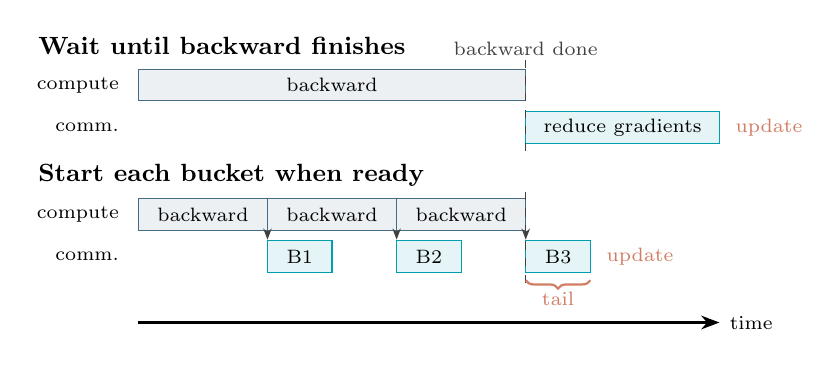
\begin{tikzpicture}[x=.82cm,y=.67cm,every node/.style={font=\scriptsize},
    compute/.style={draw=themebluedraw,fill=themebluecard},
    comm/.style={draw=accentdarkdraw,fill=accentdarkbg},
    ready/.style={-{Stealth[length=4pt,width=3pt]},thick,draw=neutraldark}]
    % Same illustrative backward and communication work in each scenario.
    \node[anchor=west,font=\small\bfseries] at (-1.7,4.9) {Wait until backward finishes};
    \node[anchor=east] at (-.15,4.15) {compute};
    \node[anchor=east] at (-.15,3.35) {comm.};
    \draw[compute] (0,3.85) rectangle (6,4.45);
    \node at (3,4.15) {backward};
    \draw[comm] (6,3.05) rectangle (9,3.65);
    \node at (7.5,3.35) {reduce gradients};
    \draw[dashed,neutraldark] (6,2.9)--(6,4.65);
    \node[anchor=west,text=leafreddraw] at (9.1,3.35) {update};
    \node[font=\scriptsize,text=neutraldark,anchor=south] at (6,4.52) {backward done};
    \node[anchor=west,font=\small\bfseries] at (-1.7,2.45) {Start each bucket when ready};
    \node[anchor=east] at (-.15,1.7) {compute};
    \node[anchor=east] at (-.15,.9) {comm.};
    \draw[compute] (0,1.4) rectangle (2,2);
    \draw[compute] (2,1.4) rectangle (4,2);
    \draw[compute] (4,1.4) rectangle (6,2);
    \node at (1,1.7) {backward};
    \node at (3,1.7) {backward};
    \node at (5,1.7) {backward};
    \draw[comm] (2,.6) rectangle (3,1.2); \node at (2.5,.9) {B1};
    \draw[comm] (4,.6) rectangle (5,1.2); \node at (4.5,.9) {B2};
    \draw[comm] (6,.6) rectangle (7,1.2); \node at (6.5,.9) {B3};
    \draw[ready] (2,1.38)--(2,1.22); \draw[ready] (4,1.38)--(4,1.22); \draw[ready] (6,1.38)--(6,1.22);
    \draw[dashed,neutraldark] (6,.4)--(6,2.2);
    \draw[decorate,decoration={brace,amplitude=3pt,mirror},draw=leafreddraw,thick] (6,.45)--(7,.45);
    \node[text=leafreddraw,anchor=west] at (7.1,.9) {update};
    \node[text=leafreddraw] at (6.5,.1) {tail};
    \draw[-{Stealth},thick] (0,-.35)--(9,-.35) node[right]{time};
  \end{tikzpicture}
  \end{center}
  \footnotesize B1--B3 are gradient buckets. Only the final reduction remains after backward; the update waits for it. Timings are illustrative.
\end{frame}

\begin{frame}{Distributed sampling is part of correctness}
  \begin{itemize}
      \setlength{\itemsep}{8pt}
    \item Each rank needs a disjoint subset within an epoch or sampling interval.
    \item All ranks must agree on the shuffle seed and epoch counter.
    \item Dropping or padding the tail changes sample multiplicity.
    \item Resume must restore the sampler's logical position.
  \end{itemize}
  \begin{block}{Fast audit}
    Log sample IDs per rank for a few updates. Check within-step overlap, missing examples, and resume continuity.
  \end{block}
\end{frame}

\begin{frame}{Only some side effects should happen on every rank}
  \small
  \begin{tabular}{lll}
    \toprule
    Action & Every rank? & Reason \\
    \midrule
    forward and backward & yes & local data contribution \\
    optimizer update & yes & replicas remain identical \\
    metric numerator/count & yes & later reduction \\
    console and tracker logging & usually rank 0 & avoid duplicates \\
    full checkpoint publication & coordinated & avoid corruption \\
    validation sampling & sharded or rank 0 & declare aggregation \\
    \bottomrule
  \end{tabular}
\end{frame}

\checkpoint{batch accounting}
{With $W=8$, micro-batch 2, context 2048, and four accumulated micro-steps, compute tokens per update. How many gradient synchronizations should occur?}

\section{Correctness before scaling}

\begin{frame}{A five-rung correctness ladder}
  \begin{enumerate}
      \setlength{\itemsep}{5pt}
    \item parameters are identical immediately after initialization
    \item one global-batch update matches a single-process reference
    \item parameters remain synchronized after the update
    \item sample IDs show the intended global data coverage
    \item save and resume preserve model, optimizer, RNG, and sampler state
  \end{enumerate}
  \begin{alertblock}{Tolerance is part of the test}
    Reduction order changes floating-point rounding. Define acceptable numerical error rather than demanding bitwise equality by accident.
  \end{alertblock}
\end{frame}

\begin{frame}{Scaling efficiency separates speed from more work}
  \[
    \text{speedup}(W)=\frac{t_1}{t_W},
    \qquad
    \text{efficiency}(W)=\frac{\text{speedup}(W)}{W}
  \]
  \begin{columns}[t]
    \begin{column}{0.47\linewidth}
      \begin{block}{Strong scaling}
        Hold the global batch and work fixed. Ask how much faster the same update becomes.
      \end{block}
    \end{column}
    \begin{column}{0.47\linewidth}
      \begin{block}{Weak scaling}
        Hold work per GPU fixed. Global batch grows with $W$.
      \end{block}
    \end{column}
  \end{columns}
\end{frame}

\begin{frame}{A trace explains poor scaling}
  \begin{itemize}
      \setlength{\itemsep}{7pt}
    \item long exposed collectives suggest insufficient compute overlap or slow links
    \item rank skew suggests data loading, imbalance, or stragglers
    \item many small collectives suggest poor bucketing
    \item gaps before collectives suggest autograd readiness or synchronization barriers
    \item identical time with more GPUs may mean the local batch became too small
  \end{itemize}
\end{frame}

\checkpoint{equivalence failure}
{A two-GPU run has the expected throughput, but its first update differs sharply from the single-process reference. Give a check order covering initialization, data, loss normalization, reduction, and optimizer state.}

\takeaways
{DDP is equivalent to a global mean update only when data and normalization invariants hold.}
{Collective communication has startup and bandwidth costs; buckets can overlap it with backward.}
{Sampling, metrics, side effects, and resume logic must all understand rank.}
{Correctness comparisons come before speedup and efficiency measurements.}
\end{document}
